\begin{frame}{Observations on Chasing the Lights}
	The window of influence
	\bigskip
	\begin{columns}
		\begin{column}{0.45\linewidth}
			\includegraphics[width=\textwidth]{image/window-0.ps}
		\end{column}
		\begin{column}{0.45\linewidth}
			\includegraphics[width=\textwidth]{image/window-1.ps}
		\end{column}
	\end{columns}
\end{frame}

\begin{frame}{Modelling the Window}
	\begin{columns}
		\begin{column}{0.45\linewidth}
			\includegraphics[width=\textwidth]{image/window-0.ps}
		\end{column}
		\begin{column}{0.45\linewidth}
			\[
				\left(
				\begin{array}{c}
					1 \\
					1 \\
					1 \\
					0 \\
					0 \\
					0 \\
					1 \\
					0 \\
					0 \\
					0 \\
				\end{array}
				\right) \in \GF(2)^{10}
			\]
		\end{column}
	\end{columns}
	
\end{frame}

\begin{frame}{Windowing Transformation}
	\begin{columns}[T]
		\begin{column}{0.45\linewidth}
			Let $c$ be the number of columns
			
			\bigskip
			
			\begin{definition}
				$W_{c} : \GF(2)^{2c} \rightarrow \GF(2)^{2c}$ is called
				a \structure{windowing transformation}.
			\end{definition}
			
			\bigskip
			
			\begin{theorem}
				$W_{c}$ is a linear transformation for all $c \in \N^{*}$
			\end{theorem}
		\end{column}
		\begin{column}{0.45\linewidth}
			\[
				W_{c} := \left(
				\begin{tabular}{cc}
					$E_{c}$ & $I$ \\
					$I$ & $O$ \\
				\end{tabular}
				\right)
			\]
			where
			\[
				E_{5} := \left(
				\begin{tabular}{ccccc}
					1 & 1 & 0 & 0 & 0 \\
					1 & 1 & 1 & 0 & 0 \\
					0 & 1 & 1 & 1 & 0 \\
					0 & 0 & 1 & 1 & 1 \\
					0 & 0 & 0 & 1 & 1 \\
				\end{tabular}
				\right)
			\]
		\end{column}
	\end{columns}
\end{frame}

\begin{frame}{Windowing Transformation}
	\begin{lemma}
		$W_{c}$ is invertable for all $c \in \N^{*}$
	\end{lemma}
	
	\pause
	\bigskip
	
	\begin{proof}
		\[
			\left(
			\begin{tabular}{cc}
				$E$ & $I$ \\
				$I$ & $O$ \\
			\end{tabular}
			\right)
			\cdot
			\left(
			\begin{tabular}{cc}
				$O$ & $I$ \\
				$I$ & $-E$ \\
			\end{tabular}
			\right)
			=
			\left(
			\begin{tabular}{cc}
				$I$ & $O$ \\
				$O$ & $I$ \\
			\end{tabular}			
			\right)
		\]
	\end{proof}
\end{frame}

\begin{frame}{Windowing Transformation}
	\begin{theorem}
		The sequence $W_{c}^{0}, W_{c}^{1}, W_{c}^{2}, W_{c}^{3}, \ldots$ is periodic
	\end{theorem}
	
	\pause
	\bigskip
	
	\begin{proof}
		There are finitely many square matrices of size $c$ over $\GF(2)$
		
		The sequence $W_{c}^{0}, W_{c}^{1}, W_{c}^{2},\ldots$ must repeat
		
		By the preceding lemma $W_{c}$ is invertable
		
		This proves the periodicity of the above sequence
	\end{proof}
	
	\pause
	\bigskip
	
	\begin{corollary}
		The sequence of left upper submatrices of 
		$W_{c}^{0}, W_{c}^{1}, W_{c}^{2},\ldots$ is periodic
	\end{corollary}
\end{frame}
